\documentclass{article}\usepackage[]{graphicx}\usepackage[]{color}
%% maxwidth is the original width if it is less than linewidth
%% otherwise use linewidth (to make sure the graphics do not exceed the margin)
\makeatletter
\def\maxwidth{ %
  \ifdim\Gin@nat@width>\linewidth
    \linewidth
  \else
    \Gin@nat@width
  \fi
}
\makeatother

\definecolor{fgcolor}{rgb}{0.345, 0.345, 0.345}
\newcommand{\hlnum}[1]{\textcolor[rgb]{0.686,0.059,0.569}{#1}}%
\newcommand{\hlstr}[1]{\textcolor[rgb]{0.192,0.494,0.8}{#1}}%
\newcommand{\hlcom}[1]{\textcolor[rgb]{0.678,0.584,0.686}{\textit{#1}}}%
\newcommand{\hlopt}[1]{\textcolor[rgb]{0,0,0}{#1}}%
\newcommand{\hlstd}[1]{\textcolor[rgb]{0.345,0.345,0.345}{#1}}%
\newcommand{\hlkwa}[1]{\textcolor[rgb]{0.161,0.373,0.58}{\textbf{#1}}}%
\newcommand{\hlkwb}[1]{\textcolor[rgb]{0.69,0.353,0.396}{#1}}%
\newcommand{\hlkwc}[1]{\textcolor[rgb]{0.333,0.667,0.333}{#1}}%
\newcommand{\hlkwd}[1]{\textcolor[rgb]{0.737,0.353,0.396}{\textbf{#1}}}%

\usepackage{framed}
\makeatletter
\newenvironment{kframe}{%
 \def\at@end@of@kframe{}%
 \ifinner\ifhmode%
  \def\at@end@of@kframe{\end{minipage}}%
  \begin{minipage}{\columnwidth}%
 \fi\fi%
 \def\FrameCommand##1{\hskip\@totalleftmargin \hskip-\fboxsep
 \colorbox{shadecolor}{##1}\hskip-\fboxsep
     % There is no \\@totalrightmargin, so:
     \hskip-\linewidth \hskip-\@totalleftmargin \hskip\columnwidth}%
 \MakeFramed {\advance\hsize-\width
   \@totalleftmargin\z@ \linewidth\hsize
   \@setminipage}}%
 {\par\unskip\endMakeFramed%
 \at@end@of@kframe}
\makeatother

\definecolor{shadecolor}{rgb}{.97, .97, .97}
\definecolor{messagecolor}{rgb}{0, 0, 0}
\definecolor{warningcolor}{rgb}{1, 0, 1}
\definecolor{errorcolor}{rgb}{1, 0, 0}
\newenvironment{knitrout}{}{} % an empty environment to be redefined in TeX

\usepackage{alltt}

\usepackage[margin = 0.5in]{geometry}
\usepackage{float, enumitem}
\usepackage{graphicx}
\usepackage{amsmath}

\setlength{\topsep}{0pt}
\setlength{\parskip}{0pt}
\setlength{\partopsep}{1pt}

\renewcommand\thesubsection{\thesection (\alph{subsection})}
\IfFileExists{upquote.sty}{\usepackage{upquote}}{}
\begin{document}

\title{ASSIGNMENT 6}
\author{Brandon Lampe \\ STAT 527 \\ Advanced Data Analysis I}
\maketitle



\section{Parallax:}
\begin{knitrout}
\definecolor{shadecolor}{rgb}{0.969, 0.969, 0.969}\color{fgcolor}\begin{kframe}
\begin{alltt}
\hlcom{#  load all data for assignment and write to .csv files because website download}
\hlcom{#  is not reliable}
\hlstd{dir} \hlkwb{<-} \hlkwd{getwd}\hlstd{()} \hlcom{# current directory}
\hlcom{# parallax <- read.csv("http://statacumen.com/teach/ADA1/ADA1_HW_06_F14-1.csv")}
\hlcom{# write.table(parallax, paste(dir, "p1.csv", sep = "/"), sep = ",", row.names = FALSE )}
\hlstd{parallax} \hlkwb{<-} \hlkwd{read.csv}\hlstd{(}\hlkwd{paste}\hlstd{(dir,} \hlstr{"p1.csv"}\hlstd{,} \hlkwc{sep} \hlstd{=} \hlstr{"/"}\hlstd{))}
\hlstd{angle} \hlkwb{<-} \hlstd{parallax}\hlopt{$}\hlstd{angle;}
\end{alltt}
\end{kframe}
\end{knitrout}

\begin{knitrout}
\definecolor{shadecolor}{rgb}{0.969, 0.969, 0.969}\color{fgcolor}\begin{kframe}
\begin{alltt}
\hlkwd{summary}\hlstd{(angle)}
\end{alltt}
\begin{verbatim}
##    Min. 1st Qu.  Median    Mean 3rd Qu.    Max. 
##   5.760   8.340   8.500   8.616   9.020  10.570
\end{verbatim}
\begin{alltt}
\hlkwd{sd}\hlstd{(angle)} \hlcom{# standard deviation}
\end{alltt}
\begin{verbatim}
## [1] 0.7490205
\end{verbatim}
\begin{alltt}
\hlkwd{max}\hlstd{(angle)} \hlopt{-} \hlkwd{min}\hlstd{(angle)} \hlcom{#spread}
\end{alltt}
\begin{verbatim}
## [1] 4.81
\end{verbatim}
\begin{alltt}
\hlkwd{fivenum}\hlstd{(angle)[}\hlnum{4}\hlstd{]} \hlopt{-} \hlkwd{fivenum}\hlstd{(angle)[}\hlnum{2}\hlstd{]} \hlcom{#IQR}
\end{alltt}
\begin{verbatim}
## [1] 0.68
\end{verbatim}
\end{kframe}
\end{knitrout}

\begin{knitrout}
\definecolor{shadecolor}{rgb}{0.969, 0.969, 0.969}\color{fgcolor}\begin{kframe}
\begin{alltt}
\hlcom{#create box plot}
\hlstd{angle.hist} \hlkwb{<-} \hlkwd{ggplot}\hlstd{(parallax,} \hlkwd{aes}\hlstd{(}\hlkwc{x} \hlstd{= angle))}
\hlstd{angle.hist} \hlkwb{<-} \hlstd{angle.hist} \hlopt{+} \hlkwd{geom_histogram}\hlstd{(}\hlkwd{aes}\hlstd{(}\hlkwc{y} \hlstd{= ..density..),}
                                          \hlkwc{binwidth} \hlstd{=} \hlnum{.25}\hlstd{,}\hlkwc{color} \hlstd{=} \hlstr{"black"}\hlstd{,} \hlkwc{fill} \hlstd{=} \hlstr{"white"}\hlstd{)}
\hlstd{angle.hist} \hlkwb{<-} \hlstd{angle.hist} \hlopt{+} \hlkwd{geom_density}\hlstd{(}\hlkwc{alpha} \hlstd{=} \hlnum{0.2}\hlstd{,} \hlkwc{fill} \hlstd{=} \hlstr{"#FF6666"}\hlstd{)}
\hlstd{angle.hist} \hlkwb{<-} \hlstd{angle.hist} \hlopt{+} \hlkwd{labs}\hlstd{(}\hlkwc{x} \hlstd{=} \hlstr{"angle"}\hlstd{)}

\hlcom{# boxplot of angle}
\hlstd{angle.box} \hlkwb{<-} \hlkwd{ggplot}\hlstd{(parallax,} \hlkwd{aes}\hlstd{(}\hlkwc{x} \hlstd{=} \hlstr{"angle"}\hlstd{,} \hlkwc{y} \hlstd{= angle))} \hlcom{# boxplot of angle}
\hlstd{angle.box} \hlkwb{<-} \hlstd{angle.box} \hlopt{+} \hlkwd{geom_boxplot}\hlstd{()}
\hlstd{angle.box} \hlkwb{<-} \hlstd{angle.box} \hlopt{+} \hlkwd{coord_flip}\hlstd{()}
\hlstd{angle.box} \hlkwb{<-} \hlstd{angle.box} \hlopt{+} \hlkwd{labs}\hlstd{(}\hlkwc{x} \hlstd{=} \hlstr{""}\hlstd{,} \hlkwc{y} \hlstd{=} \hlstr{"angle"}\hlstd{)}
\hlstd{angle.box} \hlkwb{<-} \hlstd{angle.box} \hlopt{+} \hlkwd{stat_summary}\hlstd{(}\hlkwc{fun.y} \hlstd{= mean,} \hlkwc{geom} \hlstd{=} \hlstr{"point"}\hlstd{,} \hlkwc{shape} \hlstd{=} \hlnum{3}\hlstd{,} \hlkwc{size} \hlstd{=} \hlnum{4}\hlstd{)}
\hlcom{# plot}
\hlkwd{grid.arrange}\hlstd{(angle.hist, angle.box,} \hlkwc{nrow} \hlstd{=} \hlnum{2}\hlstd{)}
\end{alltt}
\end{kframe}

{\centering 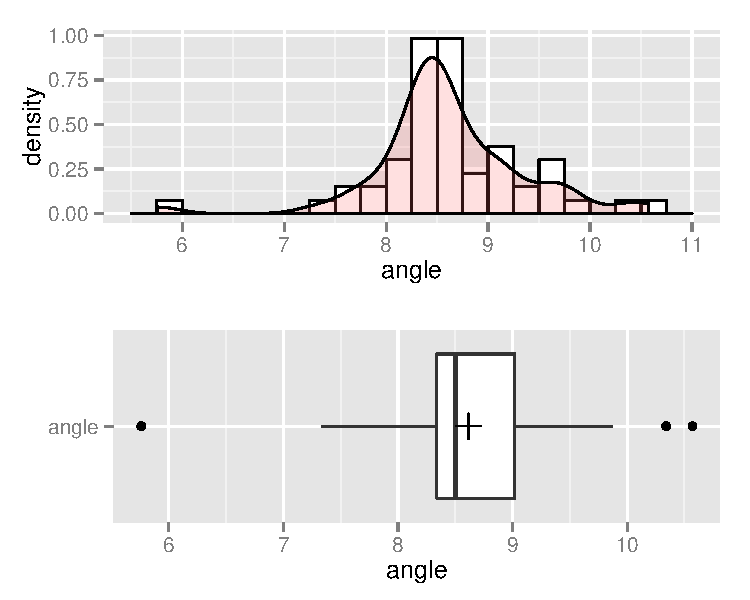
\includegraphics[width=\maxwidth]{figure/1_a-1} 

}



\end{knitrout}

\begin{knitrout}
\definecolor{shadecolor}{rgb}{0.969, 0.969, 0.969}\color{fgcolor}\begin{kframe}
\begin{alltt}
\hlkwd{bs.one.samp.dist}\hlstd{(angle)} \hlcom{# bootstrap}
\hlkwd{qqPlot}\hlstd{(angle)}
\end{alltt}
\end{kframe}

{\centering 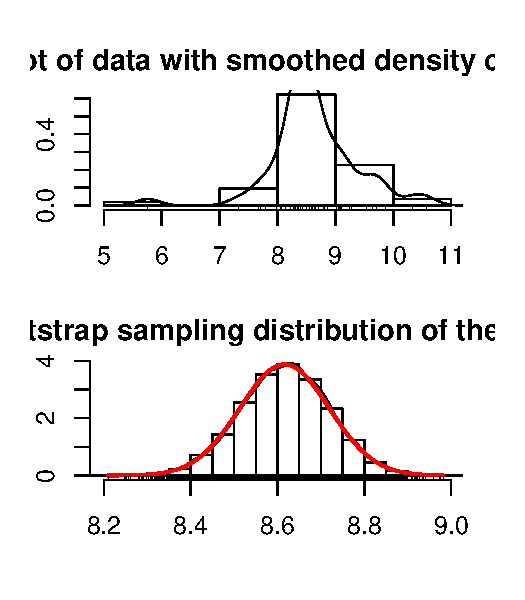
\includegraphics[width=\maxwidth]{figure/1_a_boot-1} 
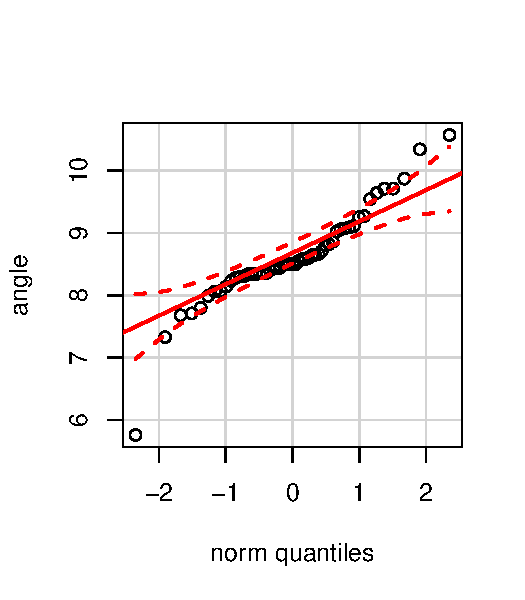
\includegraphics[width=\maxwidth]{figure/1_a_boot-2} 

}



\end{knitrout}

\subsection{(5 pts) Describe the distribution of determinations of the parallax. Be complete.}
The distribution of measurements of the parallax using Short's device is unimodal and has
a standard deviation that is approximately equal to the IQR.  The data do not appear
 symmetric.
Also, the data contains extreme outiers on both left and right sides
and has tails of nearly equal length.
The bootstrap sampling distribution of the mean parallax angle using Short's device appears
symmetric and normal.  The Q-Q plot shows that the data fall within the range of a
normal distribution except for the extreme outliers on the left and right sides, which cause the mean to be
greater than the median.\


\subsection{(10 pts) Perform the standard t-test on these data, at the 5% level, and construct a 95% CI for μ.
Interpret the results, given the question of interest.}
\begin{knitrout}
\definecolor{shadecolor}{rgb}{0.969, 0.969, 0.969}\color{fgcolor}\begin{kframe}
\begin{alltt}
\hlcom{# t-test}
\hlstd{angle.t} \hlkwb{<-} \hlkwd{t.test}\hlstd{(angle,} \hlkwc{mu} \hlstd{=} \hlnum{8.798}\hlstd{,} \hlkwc{conf.level} \hlstd{=} \hlnum{0.95}\hlstd{)}
\hlstd{angle.t}
\end{alltt}
\begin{verbatim}
## 
## 	One Sample t-test
## 
## data:  angle
## t = -1.7667, df = 52, p-value = 0.08314
## alternative hypothesis: true mean is not equal to 8.798
## 95 percent confidence interval:
##  8.409771 8.822682
## sample estimates:
## mean of x 
##  8.616226
\end{verbatim}
\begin{alltt}
\hlkwd{diff}\hlstd{(angle.t}\hlopt{$}\hlstd{conf.int)} \hlcom{#width of CI}
\end{alltt}
\begin{verbatim}
## [1] 0.4129112
\end{verbatim}
\end{kframe}
\end{knitrout}

We are interested in if it is plausible that the mean of all potential measurements using
Short's device agrees with the currently accepted parallax value of 8.798.  In notation,
$H_0: \mu = 8.798$ against $H_A: \mu \ne 8.798$.  The one sample t-test results in a p-value
 of 0.08, which is greater than 0.05, and a 95\% confidence interval of 8.41 to 8.82, which
 includes 8.798.  Therefore, based on these results it is plausible for the population mean
 of all potential measurements of the parallax using Short's device to equal 8.798, and I fail
 to reject the null.

\subsection{(10 pts) Repeat the analysis using a suitable non-parametric method, and contrast the results with
part (b). Which analysis seems most reasonable, and what are your conclusions based on that analysis, given the question of interest?}

\begin{knitrout}
\definecolor{shadecolor}{rgb}{0.969, 0.969, 0.969}\color{fgcolor}\begin{kframe}
\begin{alltt}
\hlcom{# sign test}
\hlstd{sign.t} \hlkwb{<-} \hlkwd{SIGN.test}\hlstd{(angle,} \hlkwc{md} \hlstd{=} \hlnum{8.798}\hlstd{)}
\end{alltt}
\begin{verbatim}
## 
## 	One-sample Sign-Test
## 
## data:  angle
## s = 17, p-value = 0.01266
## alternative hypothesis: true median is not equal to 8.798
## 95 percent confidence interval:
##  8.394796 8.651301
## sample estimates:
## median of x 
##         8.5
\end{verbatim}
\begin{alltt}
\hlstd{sign.t}
\end{alltt}
\begin{verbatim}
##                   Conf.Level L.E.pt U.E.pt
## Lower Achieved CI     0.9466 8.4000 8.6500
## Interpolated CI       0.9500 8.3948 8.6513
## Upper Achieved CI     0.9730 8.3600 8.6600
\end{verbatim}
\begin{alltt}
\hlkwd{diff}\hlstd{(sign.t[}\hlnum{2}\hlstd{,}\hlkwd{c}\hlstd{(}\hlnum{2}\hlstd{,}\hlnum{3}\hlstd{)])} \hlcom{# width of CI}
\end{alltt}
\begin{verbatim}
## U.E.pt 
## 0.2565
\end{verbatim}
\begin{alltt}
\hlcom{#wilcoxon test}
\hlstd{w.t} \hlkwb{<-} \hlkwd{wilcox.test}\hlstd{(angle,} \hlkwc{mu} \hlstd{=} \hlnum{8.798}\hlstd{,} \hlkwc{conf.int} \hlstd{=} \hlnum{TRUE}\hlstd{)}
\hlstd{w.t}
\end{alltt}
\begin{verbatim}
## 
## 	Wilcoxon signed rank test with continuity correction
## 
## data:  angle
## V = 465, p-value = 0.02686
## alternative hypothesis: true location is not equal to 8.798
## 95 percent confidence interval:
##  8.430072 8.774983
## sample estimates:
## (pseudo)median 
##       8.574997
\end{verbatim}
\begin{alltt}
\hlkwd{diff}\hlstd{(w.t}\hlopt{$}\hlstd{conf.int)} \hlcom{#width of CI}
\end{alltt}
\begin{verbatim}
## [1] 0.3449107
\end{verbatim}
\end{kframe}
\end{knitrout}
The sign test determines if it is plausible that the median of all potential measurements using
Short's device agrees with the currently accepted parallax value of 8.798.  In notation,
$H_0: \eta = 8.798$ against $H_A: \eta \ne 8.798$.  The sign test results in a p-value
 of 0.01, which is less than 0.05, and an interpolated 95\% confidence interval of 8.39 to 8.65, which
 does not include 8.798.  Therefore, based on these results it is not plausible for the population median
 of all potential measurements of the parallax using Short's device to equal 8.798, and I
 reject the null in favor of the alternative.\

 The Wilcoxon procedure test determines if it is plausible that the mean of all potential measurements using
Short's device agrees with the currently accepted parallax value of 8.798.  In notation,
$H_0: \mu = 8.798$ against $H_A: \mu \ne 8.798$.  The Wilcoxon test results in a p-value
 of 0.03, which is less than 0.05, and an interpolated 95\% confidence interval of 8.430 to 8.775, which
 does not include 8.798.  Therefore, based on these results it is not plausible for the population mean
 of all potential measurements of the parallax using Short's device to equal 8.798, and I
 reject the null in favor of the alternative.

 \begin{itemize}
 \item (b):  I believe the t-test is the most reasonable for this analysis because the
 question of interest is in regards to the population mean, which is the parameter evaluated
 by the t-test.
 The normality assumption of the t-test appears to be valid.  The sign and Wilcoxon tests
 do not use the mean as a parameter, rather they are with respect to the median.  Additionally,
 the median is considerably far from the mean based on the IQR.  The Wilcoxon test assumes
 the sample distribution is symmetric, which this is not true based on the difference between
 the mean and median.

\end{itemize}

\section{Guinea pigs:}
\begin{knitrout}
\definecolor{shadecolor}{rgb}{0.969, 0.969, 0.969}\color{fgcolor}\begin{kframe}
\begin{alltt}
\hlcom{# guinea <- read.csv("http://statacumen.com/teach/ADA1/ADA1_HW_06_F14-2.csv")}
\hlcom{# write.table(guinea, paste(dir, "p2.csv", sep = "/"), sep = ",", row.names = FALSE )}
\hlstd{guinea} \hlkwb{<-} \hlkwd{read.csv}\hlstd{(}\hlkwd{paste}\hlstd{(dir,} \hlstr{"p2.csv"}\hlstd{,} \hlkwc{sep} \hlstd{=} \hlstr{"/"}\hlstd{))}
\hlstd{hours} \hlkwb{<-} \hlstd{guinea}\hlopt{$}\hlstd{hours}
\end{alltt}
\end{kframe}
\end{knitrout}

\begin{knitrout}
\definecolor{shadecolor}{rgb}{0.969, 0.969, 0.969}\color{fgcolor}\begin{kframe}
\begin{alltt}
\hlkwd{summary}\hlstd{(hours)}
\end{alltt}
\begin{verbatim}
##    Min. 1st Qu.  Median    Mean 3rd Qu.    Max. 
##   43.00   82.75  102.50  141.80  149.20  598.00
\end{verbatim}
\begin{alltt}
\hlkwd{sd}\hlstd{(hours)} \hlcom{# standard deviation}
\end{alltt}
\begin{verbatim}
## [1] 109.2086
\end{verbatim}
\begin{alltt}
\hlkwd{max}\hlstd{(hours)} \hlopt{-} \hlkwd{min}\hlstd{(hours)} \hlcom{#spread}
\end{alltt}
\begin{verbatim}
## [1] 555
\end{verbatim}
\begin{alltt}
\hlkwd{fivenum}\hlstd{(hours)[}\hlnum{4}\hlstd{]} \hlopt{-} \hlkwd{fivenum}\hlstd{(hours)[}\hlnum{2}\hlstd{]} \hlcom{#IQR}
\end{alltt}
\begin{verbatim}
## [1] 69
\end{verbatim}
\end{kframe}
\end{knitrout}

\begin{knitrout}
\definecolor{shadecolor}{rgb}{0.969, 0.969, 0.969}\color{fgcolor}\begin{kframe}
\begin{alltt}
\hlcom{#create box plot}
\hlstd{hours.hist} \hlkwb{<-} \hlkwd{ggplot}\hlstd{(guinea,} \hlkwd{aes}\hlstd{(}\hlkwc{x} \hlstd{= hours))}
\hlstd{hours.hist} \hlkwb{<-} \hlstd{hours.hist} \hlopt{+} \hlkwd{geom_histogram}\hlstd{(}\hlkwd{aes}\hlstd{(} \hlkwc{y}\hlstd{= ..density..),}
                                          \hlkwc{binwidth} \hlstd{=} \hlnum{25}\hlstd{,}\hlkwc{color} \hlstd{=} \hlstr{"black"}\hlstd{,} \hlkwc{fill} \hlstd{=} \hlstr{"white"}\hlstd{)}
\hlstd{hours.hist} \hlkwb{<-} \hlstd{hours.hist} \hlopt{+} \hlkwd{geom_density}\hlstd{(}\hlkwc{alpha} \hlstd{=} \hlnum{0.2}\hlstd{,} \hlkwc{fill} \hlstd{=} \hlstr{"#FF6666"}\hlstd{)}
\hlstd{hours.hist} \hlkwb{<-} \hlstd{hours.hist} \hlopt{+} \hlkwd{labs}\hlstd{(}\hlkwc{x} \hlstd{=} \hlstr{"hours"}\hlstd{)}

\hlcom{# boxplot of hours}
\hlstd{hours.box} \hlkwb{<-} \hlkwd{ggplot}\hlstd{(guinea,} \hlkwd{aes}\hlstd{(}\hlkwc{x} \hlstd{=} \hlstr{"hours"}\hlstd{,} \hlkwc{y} \hlstd{= hours))} \hlcom{# boxplot of hours}
\hlstd{hours.box} \hlkwb{<-} \hlstd{hours.box} \hlopt{+} \hlkwd{geom_boxplot}\hlstd{()}
\hlstd{hours.box} \hlkwb{<-} \hlstd{hours.box} \hlopt{+} \hlkwd{coord_flip}\hlstd{()}
\hlstd{hours.box} \hlkwb{<-} \hlstd{hours.box} \hlopt{+} \hlkwd{labs}\hlstd{(}\hlkwc{x} \hlstd{=} \hlstr{""}\hlstd{,} \hlkwc{y} \hlstd{=} \hlstr{"hours"}\hlstd{)}
\hlstd{hours.box} \hlkwb{<-} \hlstd{hours.box} \hlopt{+} \hlkwd{stat_summary}\hlstd{(}\hlkwc{fun.y} \hlstd{= mean,} \hlkwc{geom} \hlstd{=} \hlstr{"point"}\hlstd{,} \hlkwc{shape} \hlstd{=} \hlnum{3}\hlstd{,} \hlkwc{size} \hlstd{=} \hlnum{4}\hlstd{)}
\hlcom{# plot}
\hlkwd{grid.arrange}\hlstd{(hours.hist, hours.box,} \hlkwc{nrow} \hlstd{=} \hlnum{2}\hlstd{)}
\end{alltt}
\end{kframe}

{\centering 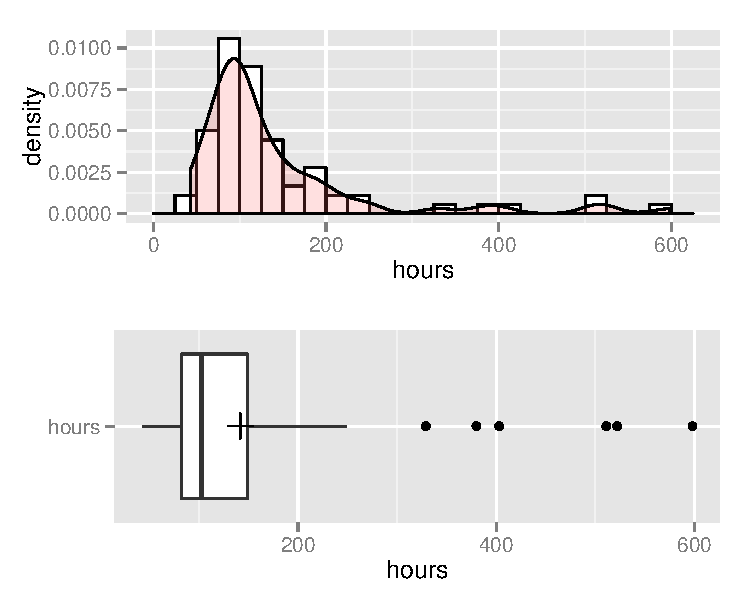
\includegraphics[width=\maxwidth]{figure/2_a_plot-1} 

}



\end{knitrout}

\begin{knitrout}
\definecolor{shadecolor}{rgb}{0.969, 0.969, 0.969}\color{fgcolor}\begin{kframe}
\begin{alltt}
\hlkwd{bs.one.samp.dist}\hlstd{(hours)} \hlcom{# bootstrap}
\hlkwd{qqPlot}\hlstd{(hours)}
\end{alltt}
\end{kframe}

{\centering 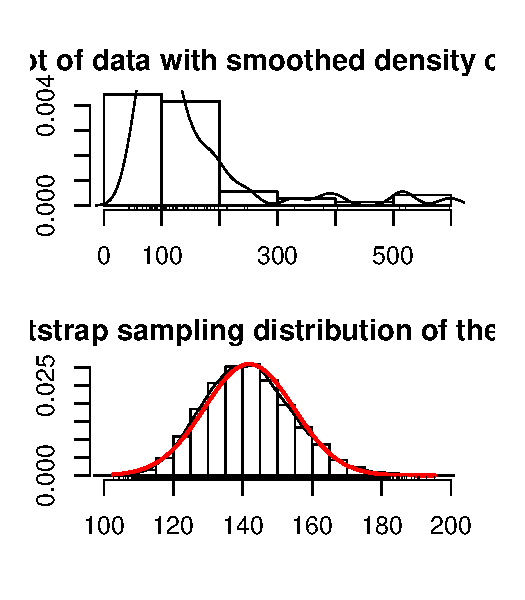
\includegraphics[width=\maxwidth]{figure/2_a_boot-1} 
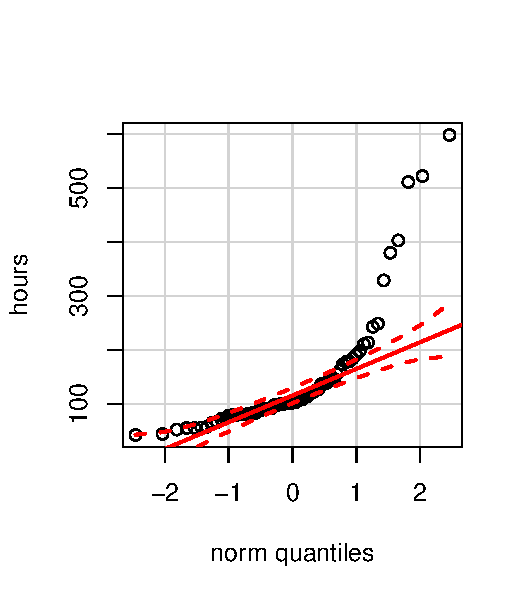
\includegraphics[width=\maxwidth]{figure/2_a_boot-2} 

}



\end{knitrout}

\subsection{(10 pts) Obtain a 95\% t-CI for the mean survival time.)}
\begin{knitrout}
\definecolor{shadecolor}{rgb}{0.969, 0.969, 0.969}\color{fgcolor}\begin{kframe}
\begin{alltt}
\hlstd{hours.t} \hlkwb{<-} \hlkwd{t.test}\hlstd{(hours,} \hlkwc{conf.level} \hlstd{=} \hlnum{0.95}\hlstd{)}
\hlstd{hours.t}
\end{alltt}
\begin{verbatim}
## 
## 	One Sample t-test
## 
## data:  hours
## t = 11.0212, df = 71, p-value < 2.2e-16
## alternative hypothesis: true mean is not equal to 0
## 95 percent confidence interval:
##  116.1845 167.5100
## sample estimates:
## mean of x 
##  141.8472
\end{verbatim}
\begin{alltt}
\hlkwd{diff}\hlstd{(hours.t}\hlopt{$}\hlstd{conf.int)}
\end{alltt}
\begin{verbatim}
## [1] 51.32554
\end{verbatim}
\end{kframe}
\end{knitrout}

We are interested in the mean survival times in hours for guinea pigs after they were injected with
a dose of tubercule bacilli.  The 95\% confidence interval, from the one sample t-test,
indicates that the mean survival time for guinea pigs after injection ranges from 116.18 to
167.51 hours.  This confidence interval has a width of 51.33 hours about the mean.

\subsection{(10 pts) Repeat part (a) using a suitable nonparametric method.)}
\begin{knitrout}
\definecolor{shadecolor}{rgb}{0.969, 0.969, 0.969}\color{fgcolor}\begin{kframe}
\begin{alltt}
\hlcom{# sign test}
\hlstd{sign.hr} \hlkwb{<-} \hlkwd{SIGN.test}\hlstd{(hours)}
\end{alltt}
\begin{verbatim}
## 
## 	One-sample Sign-Test
## 
## data:  hours
## s = 72, p-value = 6.661e-16
## alternative hypothesis: true median is not equal to 0
## 95 percent confidence interval:
##   97.35184 120.47224
## sample estimates:
## median of x 
##       102.5
\end{verbatim}
\begin{alltt}
\hlkwd{diff}\hlstd{(sign.hr[}\hlnum{2}\hlstd{,}\hlkwd{c}\hlstd{(}\hlnum{2}\hlstd{,}\hlnum{3}\hlstd{)])} \hlcom{# width of CI}
\end{alltt}
\begin{verbatim}
##  U.E.pt 
## 23.1204
\end{verbatim}
\begin{alltt}
\hlcom{# #wilcoxon test}
\hlcom{# w.hr <- wilcox.test(hours, conf.int = TRUE)}
\hlcom{# w.hr}
\hlcom{# diff(w.hr$conf.int) #width of CI}
\end{alltt}
\end{kframe}
\end{knitrout}

As seen in the boxplot, the data are skewed heavily to the right.  The difference between
the mean and median is over 50\% of the IQR.  From these observations and because the Wilcoxon test assumes
symmetry, it is not appropriate for this analysis.
The 95\% confidence interval, about the median hours of survival for guinea pigs after
injection, from the sign test is from 97.35 to
120.47 hours.  This confidence interval has a width of 23.12 hours.

\subsection{(10 pts) Take the log of survival time and find a 95\% t-CI for mean log survival time.)}
\begin{knitrout}
\definecolor{shadecolor}{rgb}{0.969, 0.969, 0.969}\color{fgcolor}\begin{kframe}
\begin{alltt}
\hlstd{hours.log} \hlkwb{<-} \hlkwd{log}\hlstd{(hours)}
\hlkwd{summary}\hlstd{(hours.log)}
\end{alltt}
\begin{verbatim}
##    Min. 1st Qu.  Median    Mean 3rd Qu.    Max. 
##   3.761   4.416   4.630   4.771   5.005   6.394
\end{verbatim}
\begin{alltt}
\hlkwd{sd}\hlstd{(hours.log)} \hlcom{# standard deviation}
\end{alltt}
\begin{verbatim}
## [1] 0.5595629
\end{verbatim}
\begin{alltt}
\hlkwd{max}\hlstd{(hours.log)} \hlopt{-} \hlkwd{min}\hlstd{(hours.log)} \hlcom{#spread}
\end{alltt}
\begin{verbatim}
## [1] 2.632391
\end{verbatim}
\begin{alltt}
\hlkwd{fivenum}\hlstd{(hours.log)[}\hlnum{4}\hlstd{]} \hlopt{-} \hlkwd{fivenum}\hlstd{(hours.log)[}\hlnum{2}\hlstd{]} \hlcom{#IQR}
\end{alltt}
\begin{verbatim}
## [1] 0.6073644
\end{verbatim}
\end{kframe}
\end{knitrout}

\begin{knitrout}
\definecolor{shadecolor}{rgb}{0.969, 0.969, 0.969}\color{fgcolor}\begin{kframe}
\begin{alltt}
\hlcom{#create box plot}
\hlstd{hours.log.hist} \hlkwb{<-} \hlkwd{ggplot}\hlstd{(guinea,} \hlkwd{aes}\hlstd{(}\hlkwc{x} \hlstd{= hours.log))}
\hlstd{hours.log.hist} \hlkwb{<-} \hlstd{hours.log.hist} \hlopt{+} \hlkwd{geom_histogram}\hlstd{(}\hlkwd{aes}\hlstd{(}\hlkwc{y} \hlstd{= ..density..),}
                                                  \hlkwc{binwidth} \hlstd{=} \hlnum{.25}\hlstd{,} \hlkwc{color} \hlstd{=} \hlstr{"black"}\hlstd{,}
                                                  \hlkwc{fill} \hlstd{=} \hlstr{"white"}\hlstd{)}
\hlstd{hours.log.hist} \hlkwb{<-} \hlstd{hours.log.hist} \hlopt{+} \hlkwd{labs}\hlstd{(}\hlkwc{x} \hlstd{=} \hlstr{"log(hours)"}\hlstd{)}
\hlstd{hours.log.hist} \hlkwb{<-} \hlstd{hours.log.hist} \hlopt{+} \hlkwd{geom_density}\hlstd{(}\hlkwc{alpha} \hlstd{=} \hlnum{0.2}\hlstd{,} \hlkwc{fill} \hlstd{=} \hlstr{"#FF6666"}\hlstd{)}

\hlcom{# boxplot of hours.log}
\hlstd{hours.log.box} \hlkwb{<-} \hlkwd{ggplot}\hlstd{(guinea,} \hlkwd{aes}\hlstd{(}\hlkwc{x} \hlstd{=} \hlstr{"log(hours)"}\hlstd{,} \hlkwc{y} \hlstd{= hours.log))} \hlcom{# boxplot of hours.log}
\hlstd{hours.log.box} \hlkwb{<-} \hlstd{hours.log.box} \hlopt{+} \hlkwd{geom_boxplot}\hlstd{()}
\hlstd{hours.log.box} \hlkwb{<-} \hlstd{hours.log.box} \hlopt{+} \hlkwd{coord_flip}\hlstd{()}
\hlstd{hours.log.box} \hlkwb{<-} \hlstd{hours.log.box} \hlopt{+} \hlkwd{labs}\hlstd{(}\hlkwc{x} \hlstd{=} \hlstr{""}\hlstd{,} \hlkwc{y} \hlstd{=} \hlstr{"log(hours)"}\hlstd{)}
\hlstd{hours.log.box} \hlkwb{<-} \hlstd{hours.log.box} \hlopt{+} \hlkwd{stat_summary}\hlstd{(}\hlkwc{fun.y} \hlstd{= mean,} \hlkwc{geom} \hlstd{=} \hlstr{"point"}\hlstd{,} \hlkwc{shape} \hlstd{=} \hlnum{3}\hlstd{,} \hlkwc{size} \hlstd{=} \hlnum{4}\hlstd{)}
\hlcom{# plot}
\hlkwd{grid.arrange}\hlstd{(hours.log.hist, hours.log.box,} \hlkwc{nrow} \hlstd{=} \hlnum{2}\hlstd{)}
\end{alltt}
\end{kframe}

{\centering 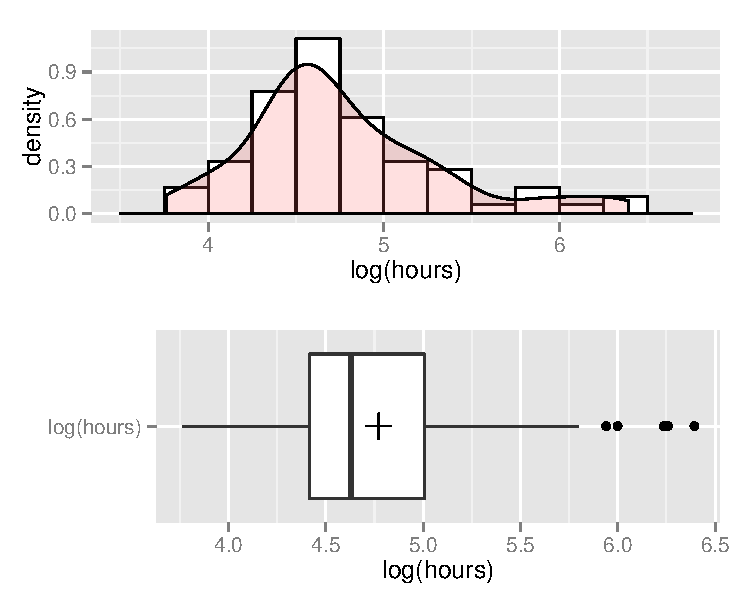
\includegraphics[width=\maxwidth]{figure/2_c-1} 

}



\end{knitrout}

\begin{knitrout}
\definecolor{shadecolor}{rgb}{0.969, 0.969, 0.969}\color{fgcolor}\begin{kframe}
\begin{alltt}
\hlkwd{bs.one.samp.dist}\hlstd{(hours.log)} \hlcom{# bootstrap}
\hlkwd{qqPlot}\hlstd{(hours.log)}
\end{alltt}
\end{kframe}

{\centering 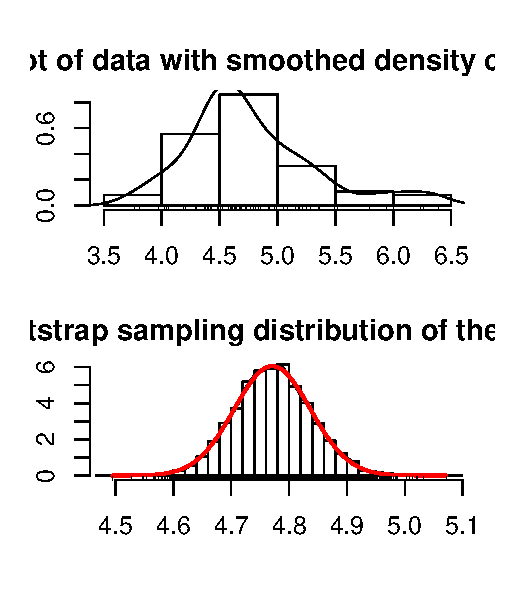
\includegraphics[width=\maxwidth]{figure/2_c_boot-1} 
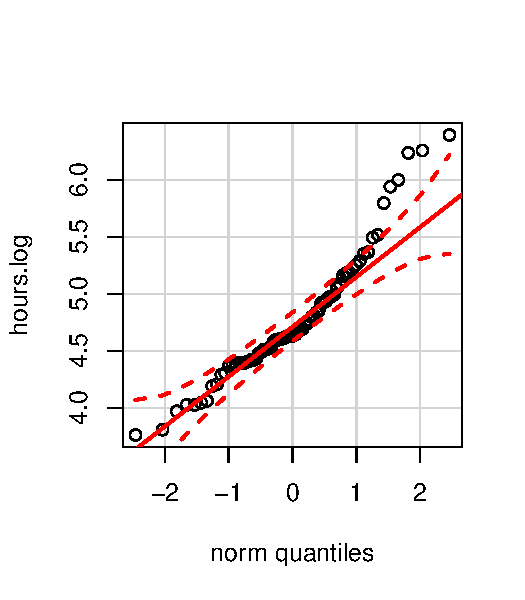
\includegraphics[width=\maxwidth]{figure/2_c_boot-2} 

}



\end{knitrout}

\begin{knitrout}
\definecolor{shadecolor}{rgb}{0.969, 0.969, 0.969}\color{fgcolor}\begin{kframe}
\begin{alltt}
\hlstd{hours.tlog} \hlkwb{<-} \hlkwd{t.test}\hlstd{(hours.log,} \hlkwc{conf.level} \hlstd{=} \hlnum{0.95}\hlstd{)}
\hlstd{hours.tlog}
\end{alltt}
\begin{verbatim}
## 
## 	One Sample t-test
## 
## data:  hours.log
## t = 72.3491, df = 71, p-value < 2.2e-16
## alternative hypothesis: true mean is not equal to 0
## 95 percent confidence interval:
##  4.639577 4.902558
## sample estimates:
## mean of x 
##  4.771067
\end{verbatim}
\begin{alltt}
\hlkwd{diff}\hlstd{(hours.tlog}\hlopt{$}\hlstd{conf.int)}
\end{alltt}
\begin{verbatim}
## [1] 0.2629817
\end{verbatim}
\end{kframe}
\end{knitrout}

The 95\% confidence interval, from the one sample t-test,
indicates that the log transformed mean survival time for guinea pigs after injection ranges from 4.64 to
4.90 log(hours).  This confidence interval has a width of 0.27 log(hours) about the mean.

\subsection{(10 pts) Repeat part (c) using a suitable nonparametric method.}
\begin{knitrout}
\definecolor{shadecolor}{rgb}{0.969, 0.969, 0.969}\color{fgcolor}\begin{kframe}
\begin{alltt}
\hlcom{# # sign test}
\hlcom{# sign.hr.log <- SIGN.test(hours.log)}
\hlcom{# diff(sign.hr.log[2,c(2,3)]) # width of CI}

\hlcom{#wilcoxon test}
\hlstd{w.hr.log} \hlkwb{<-} \hlkwd{wilcox.test}\hlstd{(hours.log,} \hlkwc{conf.int} \hlstd{=} \hlnum{TRUE}\hlstd{)}
\hlstd{w.hr.log}
\end{alltt}
\begin{verbatim}
## 
## 	Wilcoxon signed rank test with continuity correction
## 
## data:  hours.log
## V = 2628, p-value = 1.691e-13
## alternative hypothesis: true location is not equal to 0
## 95 percent confidence interval:
##  4.599833 4.842302
## sample estimates:
## (pseudo)median 
##       4.708047
\end{verbatim}
\begin{alltt}
\hlkwd{diff}\hlstd{(w.hr.log}\hlopt{$}\hlstd{conf.int)} \hlcom{#width of CI}
\end{alltt}
\begin{verbatim}
## [1] 0.2424688
\end{verbatim}
\end{kframe}
\end{knitrout}

The distribution for this test is nearly symmetric.  The difference between the mean and
median is approximately 20\% of the IQR; therefore, because it is more powerful,
the Wicoxon method will be used for
this analysis.

The 95\% confidence interval, about the log transformed median hours of survival for guinea pigs after
injection, from the Wilcoxon test is from 4.60 to
4.84 log(hours).  This confidence interval has a width of 0.24 log(hours).

\subsection{(10 pts) Compare your 4 CIs, and contrast the nonparametric with the t-CIs. If they differ much,
explain why they differ. Which analysis appears most appropriate? Explain.}

\vspace{.25in}
\begin{center}
\begin{tabular}{c c c c}
  Data Type & Analysis Method & Metric & CI \\ \hline
  Untransformed & t-test & mean & 141.85 $\pm$ 25.66 \\
  Untransformed & sign test & median & 102.5 $\pm$ 11.56 \\
  Transformed & t-test & mean & 4.77 $\pm$ 0.13 \\
  Transformed & Wilcoxon test & median & 4.71 $\pm$ 0.12 \\ \hline
\end{tabular}
\end{center}
\vspace{.1in}

\begin{itemize}

\item \textbf{Untransformed Data:}  The t-test resulted in a CI with a width of 51.33 hours
arond the mean of 141.85 hours, where the sign test resulted in a CI with a width of 23.12 hours
around the median of 102.5 hours.
The data are heavily skewed and not normal; therefore, the t-test and Wilcoxon tests are not
suitable because their respective assumptions of normality and symmetry are not satisfied.
The severe skewness of the data resulted in the mean being substantially larger than
the median, which results in the mean not being representative of typical data.
The sign test appears the most appropriate test method for evaluating the untransformed data.

\item \textbf{Transformed Data:}  The t-test resulted in a CI with a width of 0.26 log(hours)
around the mean of 4.77 log(hours), where the Wicoxon test resulted in a CI with a width of
0.24 log(hours) around the median of 4.71 log(hours).
The log transformation greatly minimized the skewness of the data, as is shown in the box
plot.  The boostrap distribution of the transformed data also appears normal.  Based on
these observations, Both the Wilcoxon and t-test assumptions are met.  The width of CI from
 the parametric and nonparametric methods are nearly equal and either method appears
  appropriate for use on the transformed data.

\end{itemize}

\section{Humerus sparrows:}

\begin{knitrout}
\definecolor{shadecolor}{rgb}{0.969, 0.969, 0.969}\color{fgcolor}\begin{kframe}
\begin{alltt}
\hlcom{# sparrows <- read.csv("http://statacumen.com/teach/ADA1/ADA1_HW_06_F14-3.csv")}
\hlcom{# write.table(sparrows, paste(dir, "p3.csv", sep = "/"), sep = ",", row.names = FALSE )}
\hlstd{sparrows} \hlkwb{<-} \hlkwd{read.csv}\hlstd{(}\hlkwd{paste}\hlstd{(dir,} \hlstr{"p3.csv"}\hlstd{,} \hlkwc{sep} \hlstd{=} \hlstr{"/"}\hlstd{))}
\hlstd{sparrows}\hlopt{$}\hlstd{survived} \hlkwb{<-} \hlkwd{factor}\hlstd{(sparrows}\hlopt{$}\hlstd{survived)}
\end{alltt}
\end{kframe}
\end{knitrout}

\subsection{(10 pts) Make appropriate graphical displays to compare the humerus lengths in the two samples}

\begin{knitrout}
\definecolor{shadecolor}{rgb}{0.969, 0.969, 0.969}\color{fgcolor}\begin{kframe}
\begin{alltt}
\hlcom{#create box plot}
\hlstd{spar.p} \hlkwb{<-} \hlkwd{ggplot}\hlstd{(sparrows,} \hlkwd{aes}\hlstd{(}\hlkwc{x} \hlstd{= survived,} \hlkwc{y} \hlstd{= humerus))}
\hlstd{spar.p} \hlkwb{<-} \hlstd{spar.p} \hlopt{+} \hlkwd{geom_hline}\hlstd{(}\hlkwc{yintercept} \hlstd{=} \hlkwd{mean}\hlstd{(sparrows}\hlopt{$}\hlstd{humerus),} \hlkwc{color} \hlstd{=} \hlstr{"black"}\hlstd{,}
                              \hlkwc{linetype} \hlstd{=} \hlstr{"dashed"}\hlstd{,} \hlkwc{size} \hlstd{=} \hlnum{0.3}\hlstd{,}  \hlkwc{alpha} \hlstd{=} \hlnum{0.5}\hlstd{)}
\hlstd{spar.p} \hlkwb{<-} \hlstd{spar.p} \hlopt{+} \hlkwd{geom_boxplot}\hlstd{(}\hlkwc{size} \hlstd{=} \hlnum{0.75}\hlstd{,} \hlkwc{alpha} \hlstd{=} \hlnum{0.5}\hlstd{)} \hlcom{# boxplot}
\hlstd{spar.p} \hlkwb{<-} \hlstd{spar.p} \hlopt{+} \hlkwd{geom_point}\hlstd{(}\hlkwc{position} \hlstd{=} \hlkwd{position_jitter}\hlstd{(}\hlkwc{w} \hlstd{=} \hlnum{0.05}\hlstd{,} \hlkwc{h} \hlstd{=} \hlnum{0}\hlstd{),}
                              \hlkwc{alpha} \hlstd{=} \hlnum{0.5}\hlstd{,} \hlkwc{size} \hlstd{=} \hlnum{2}\hlstd{)}
\hlstd{spar.p} \hlkwb{<-} \hlstd{spar.p} \hlopt{+} \hlkwd{stat_summary}\hlstd{(}\hlkwc{fun.y} \hlstd{= mean,} \hlkwc{geom} \hlstd{=} \hlstr{"point"}\hlstd{,} \hlkwc{shape} \hlstd{=} \hlnum{18}\hlstd{,}
                                \hlkwc{size} \hlstd{=} \hlnum{6}\hlstd{,} \hlkwd{aes}\hlstd{(}\hlkwc{color} \hlstd{= survived),} \hlkwc{alpha} \hlstd{=} \hlnum{0.8}\hlstd{)}
\hlstd{spar.p} \hlkwb{<-} \hlstd{spar.p} \hlopt{+} \hlkwd{stat_summary}\hlstd{(}\hlkwc{fun.data} \hlstd{=} \hlstr{"mean_cl_normal"}\hlstd{,} \hlkwc{geom} \hlstd{=} \hlstr{"errorbar"}\hlstd{,}
                                \hlkwc{width} \hlstd{=} \hlnum{.1}\hlstd{,} \hlkwd{aes}\hlstd{(}\hlkwc{color} \hlstd{= survived),} \hlkwc{alpha} \hlstd{=} \hlnum{0.8}\hlstd{)}
\hlstd{spar.p} \hlkwb{<-} \hlstd{spar.p} \hlopt{+} \hlkwd{labs}\hlstd{(}\hlkwc{y} \hlstd{=}\hlstr{"Humerus Lengths (inch/1000)"}\hlstd{,}\hlkwc{x} \hlstd{=} \hlstr{"Survived (binary)"}\hlstd{)}

\hlstd{spar.p} \hlkwb{<-} \hlstd{spar.p} \hlopt{+} \hlkwd{guides}\hlstd{(}\hlkwc{color} \hlstd{=} \hlnum{FALSE}\hlstd{)}
\hlcom{# create histograms}
\hlstd{spar.hist} \hlkwb{<-} \hlkwd{ggplot}\hlstd{(sparrows,} \hlkwd{aes}\hlstd{(}\hlkwc{x} \hlstd{= humerus))} \hlopt{+} \hlkwd{geom_histogram}\hlstd{(}\hlkwc{binwidth} \hlstd{=} \hlnum{10}\hlstd{)}
\hlstd{spar.hist} \hlkwb{<-} \hlstd{spar.hist} \hlopt{+} \hlkwd{facet_grid}\hlstd{(survived} \hlopt{~} \hlstd{.)}
\hlstd{spar.hist} \hlkwb{<-} \hlstd{spar.hist}\hlopt{+} \hlkwd{labs}\hlstd{(}\hlkwc{y} \hlstd{=} \hlstr{"Count"}\hlstd{,} \hlkwc{x} \hlstd{=} \hlstr{"Humerus Lengths (inch/1000)"}\hlstd{)}
\hlcom{# plot boxplot and historgram}
\hlkwd{grid.arrange}\hlstd{(spar.p, spar.hist,} \hlkwc{ncol} \hlstd{=} \hlnum{2}\hlstd{)}
\end{alltt}
\end{kframe}

{\centering 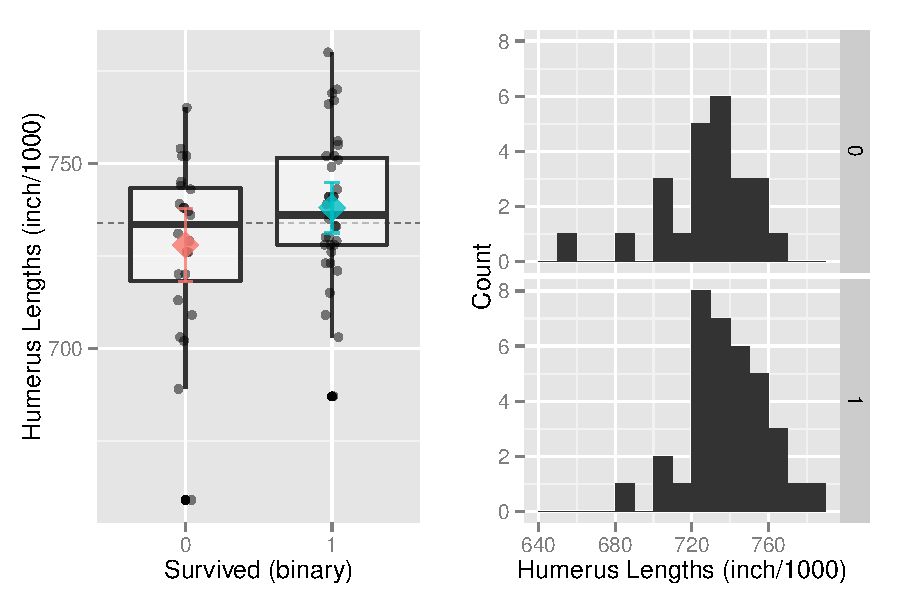
\includegraphics[width=\maxwidth]{figure/3_a_plot-1} 

}



\end{knitrout}

\begin{knitrout}
\definecolor{shadecolor}{rgb}{0.969, 0.969, 0.969}\color{fgcolor}\begin{kframe}
\begin{alltt}
\hlcom{#boostrap of the mean}
\hlstd{spar.1} \hlkwb{<-} \hlstd{sparrows[sparrows}\hlopt{$}\hlstd{survived} \hlopt{==} \hlnum{1}\hlstd{,}\hlnum{1}\hlstd{]}
\hlstd{spar.0} \hlkwb{<-} \hlstd{sparrows[sparrows}\hlopt{$}\hlstd{survived} \hlopt{!=} \hlnum{1}\hlstd{,}\hlnum{1}\hlstd{]}

\hlkwd{summary}\hlstd{(spar.1)}
\end{alltt}
\begin{verbatim}
##    Min. 1st Qu.  Median    Mean 3rd Qu.    Max. 
##   687.0   728.0   736.0   738.0   751.5   780.0
\end{verbatim}
\begin{alltt}
\hlkwd{summary}\hlstd{(spar.0)}
\end{alltt}
\begin{verbatim}
##    Min. 1st Qu.  Median    Mean 3rd Qu.    Max. 
##   659.0   718.2   733.5   727.9   743.2   765.0
\end{verbatim}
\begin{alltt}
\hlkwd{bs.two.samp.diff.dist}\hlstd{(spar.1, spar.0)}
\end{alltt}
\end{kframe}

{\centering 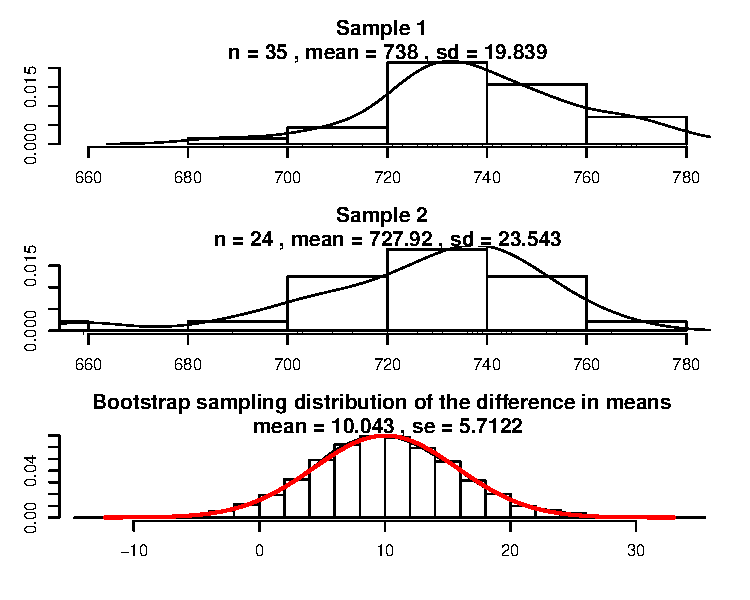
\includegraphics[width=\maxwidth]{figure/3_b_boot-1} 

}



\end{knitrout}

\subsection{(10 pts) Test at the 5\% level whether there is any difference in the population mean humerus lengths for those that perished and those that survived. Use both the t-test and an appropriate nonpara-
metric procedure.}
\begin{knitrout}
\definecolor{shadecolor}{rgb}{0.969, 0.969, 0.969}\color{fgcolor}\begin{kframe}
\begin{alltt}
\hlcom{# two sample t-test with equal variance}
\hlstd{t.spar} \hlkwb{<-} \hlkwd{t.test}\hlstd{(humerus} \hlopt{~} \hlstd{survived,} \hlkwc{data} \hlstd{= sparrows,} \hlkwc{var.equal} \hlstd{=} \hlnum{TRUE}\hlstd{)}
\hlstd{t.spar}
\end{alltt}
\begin{verbatim}
## 
## 	Two Sample t-test
## 
## data:  humerus by survived
## t = -1.777, df = 57, p-value = 0.0809
## alternative hypothesis: true difference in means is not equal to 0
## 95 percent confidence interval:
##  -21.446053   1.279386
## sample estimates:
## mean in group 0 mean in group 1 
##        727.9167        738.0000
\end{verbatim}
\begin{alltt}
\hlcom{# kruskal-Wallis test with equal variance}
\hlstd{fit.spar} \hlkwb{<-} \hlkwd{kruskal.test}\hlstd{(humerus} \hlopt{~} \hlstd{survived,} \hlkwc{data} \hlstd{= sparrows)}
\hlstd{fit.spar}
\end{alltt}
\begin{verbatim}
## 
## 	Kruskal-Wallis rank sum test
## 
## data:  humerus by survived
## Kruskal-Wallis chi-squared = 1.8881, df = 1, p-value = 0.1694
\end{verbatim}
\begin{alltt}
\hlcom{#WILCOXON-MANN-WHITNEY test of equal population dedians}
\hlkwd{wilcox.test}\hlstd{(spar.1, spar.0,} \hlkwc{conf.int} \hlstd{=} \hlnum{TRUE}\hlstd{)}
\end{alltt}
\begin{verbatim}
## 
## 	Wilcoxon rank sum test with continuity correction
## 
## data:  spar.1 and spar.0
## W = 509, p-value = 0.1718
## alternative hypothesis: true location shift is not equal to 0
## 95 percent confidence interval:
##  -3.000012 19.000020
## sample estimates:
## difference in location 
##               7.000016
\end{verbatim}
\end{kframe}
\end{knitrout}

The two sample t-test determines if it is plausible that the
difference in the mean humerus length of sparrows that died and sparrows that survived
is equal to zero.  In notation,
$H_0: \mu_1 - \mu_2 = 0$ against $H_A: \mu_1 - \mu_2 \ne 0$.  The two sample t-test resulted in a p-value
 of 0.08, which is greater than 0.05.

The Kruskal-Wallis tests if it is plausible that the
difference in the median humerus length of sparrows that died and sparrows that survived
is equal to zero.  In notation,
$H_0: \eta_1 - \eta_2 = 0$ against $H_A: \eta_1 - \eta_2 \ne 0$.  The Kruskal-Wallis test resulted in a p-value of 0.17, which
 is also greater than 0.05.  Therefore, at the 5\% level, I fail to reject the null
 hypothesis and there is no difference between
 the median humerus length of sparrows that survived and sparrows that died.

 \subsection{(10 pts) Compute and interpret a 95\% CI for the difference in population mean humerus lengths for
those that perished and those that survived. Repeat for an appropriate nonparametric procedure.}

The 95\% confidence interval from the two sample t-test for the difference in the mean
humerus length ranges from -21.45 to 1.28 (inch/1000).  The 95\% confidence interval from the
Wilcoxon-Mann-Whitney for the difference of population median humerus length resulted in a range from -3.00 to
19.00.

\subsection{(10 pts) Discuss any statistical assumptions that you have made in carrying out the analyses, and
whether the assumptions seem reasonable.}
These methods both assumed that independent random samples from two populations were utilized.
Also, the Wicoxon-Mann-Whitney test assumed that the samples came from populations having
a similar distribution, e.g., similar shaped distributions.
The two sample t-test relies on the assumption that the
distribution of the differences is normal.  Based on the plots, these assumptions
appear valid.

\subsection{(10 pts) Write a short summary for the problem. What analysis seems most appropriate?}
The two sample t-test determines if it is plausible that the
difference in the mean humerus length of sparrows that died and sparrows that survived
is equal to zero.  In notation,
$H_0: \mu_1 - \mu_2 = 0$ against $H_A: \mu_1 - \mu_2 \ne 0$.

The Kruskal-Wallis tests if it is plausible that the
difference in the median humerus length of sparrows that died and sparrows that survived
is equal to zero.  In notation,
$H_0: \eta_1 - \eta_2 = 0$ against $H_A: \eta_1 - \eta_2 \ne 0$.  The Kruskal-Wallis test resulted in a p-value of 0.17, which is greater than 0.05.  Therefore, at the 5\% level, I fail to reject the null
 hypothesis and there is no difference between
 the median humerus length of sparrows that survived and sparrows that died.

Based on the assumptions
for the respective tests, both tests appear appropriate, but the t-test assumption of normality
is the most rigorous assupmtion.  Because the two sample t-test with equal variance
has the most rigorous assumptions that are
satisified, it is the most appropriate.
The two sample t-test resulted in a p-value
 of 0.08, which is greater than 0.05.

%################################################
\section{Protoporphin levels among alcoholics:}

\begin{knitrout}
\definecolor{shadecolor}{rgb}{0.969, 0.969, 0.969}\color{fgcolor}\begin{kframe}
\begin{alltt}
\hlcom{# proto <- read.table("http://statacumen.com/teach/ADA1/ADA1_HW_06_F14-4.txt")}
\hlcom{# write.table(proto, paste(dir, "p4.csv", sep = "/"), sep = ",", row.names = FALSE )}
\hlstd{proto} \hlkwb{<-} \hlkwd{read.csv}\hlstd{(}\hlkwd{paste}\hlstd{(dir,} \hlstr{"p4.csv"}\hlstd{,} \hlkwc{sep} \hlstd{=} \hlstr{"/"}\hlstd{),} \hlkwc{header} \hlstd{=} \hlnum{TRUE}\hlstd{,} \hlkwc{stringsAsFactors} \hlstd{=} \hlnum{FALSE}\hlstd{)}
\hlstd{proto}\hlopt{$}\hlstd{row} \hlkwb{<-} \hlkwd{seq}\hlstd{(}\hlnum{1}\hlopt{:}\hlkwd{nrow}\hlstd{(proto))}
\hlstd{proto.long} \hlkwb{<-} \hlkwd{melt}\hlstd{(proto,} \hlkwc{id.vars} \hlstd{=} \hlkwd{c}\hlstd{(}\hlstr{"row"}\hlstd{),}
                   \hlkwc{measure.vars} \hlstd{=} \hlkwd{c}\hlstd{(}\hlstr{"Normal"}\hlstd{,} \hlstr{"Alc_w_sb"}\hlstd{,} \hlstr{"Alc_wo_sb"}\hlstd{),}
                   \hlkwc{variable.name} \hlstd{=} \hlstr{"type"}\hlstd{,} \hlkwc{value.name} \hlstd{=} \hlstr{"level"}\hlstd{,} \hlkwc{na.rm} \hlstd{=} \hlnum{TRUE}\hlstd{)}
\end{alltt}
\end{kframe}
\end{knitrout}

\subsection{Analysis if Untransformed Data}

\begin{knitrout}
\definecolor{shadecolor}{rgb}{0.969, 0.969, 0.969}\color{fgcolor}\begin{kframe}
\begin{alltt}
\hlcom{#create box plot}
\hlstd{proto.p} \hlkwb{<-} \hlkwd{ggplot}\hlstd{(proto.long,} \hlkwd{aes}\hlstd{(}\hlkwc{x} \hlstd{= type,} \hlkwc{y} \hlstd{= level))}
\hlstd{proto.p} \hlkwb{<-} \hlstd{proto.p} \hlopt{+} \hlkwd{geom_hline}\hlstd{(}\hlkwc{yintercept} \hlstd{=} \hlkwd{mean}\hlstd{(proto.long}\hlopt{$}\hlstd{level),} \hlkwc{color} \hlstd{=} \hlstr{"black"}\hlstd{,}
                              \hlkwc{linetype} \hlstd{=} \hlstr{"dashed"}\hlstd{,} \hlkwc{size} \hlstd{=} \hlnum{0.3}\hlstd{,}  \hlkwc{alpha} \hlstd{=} \hlnum{0.5}\hlstd{)}
\hlstd{proto.p} \hlkwb{<-} \hlstd{proto.p} \hlopt{+} \hlkwd{geom_boxplot}\hlstd{(}\hlkwc{size} \hlstd{=} \hlnum{0.75}\hlstd{,} \hlkwc{alpha} \hlstd{=} \hlnum{0.5}\hlstd{)} \hlcom{# boxplot}
\hlstd{proto.p} \hlkwb{<-} \hlstd{proto.p} \hlopt{+} \hlkwd{geom_point}\hlstd{(}\hlkwc{position} \hlstd{=} \hlkwd{position_jitter}\hlstd{(}\hlkwc{w} \hlstd{=} \hlnum{0.05}\hlstd{,} \hlkwc{h} \hlstd{=} \hlnum{0}\hlstd{),}
                              \hlkwc{alpha} \hlstd{=} \hlnum{0.5}\hlstd{,} \hlkwc{size} \hlstd{=} \hlnum{2}\hlstd{)}
\hlstd{proto.p} \hlkwb{<-} \hlstd{proto.p} \hlopt{+} \hlkwd{stat_summary}\hlstd{(}\hlkwc{fun.y} \hlstd{= mean,} \hlkwc{geom} \hlstd{=} \hlstr{"point"}\hlstd{,} \hlkwc{shape} \hlstd{=} \hlnum{18}\hlstd{,}
                                \hlkwc{size} \hlstd{=} \hlnum{6}\hlstd{,} \hlkwd{aes}\hlstd{(}\hlkwc{color} \hlstd{= type),} \hlkwc{alpha} \hlstd{=} \hlnum{0.8}\hlstd{)}
\hlstd{proto.p} \hlkwb{<-} \hlstd{proto.p} \hlopt{+} \hlkwd{stat_summary}\hlstd{(}\hlkwc{fun.data} \hlstd{=} \hlstr{"mean_cl_normal"}\hlstd{,} \hlkwc{geom} \hlstd{=} \hlstr{"errorbar"}\hlstd{,}
                                \hlkwc{width} \hlstd{=} \hlnum{.1}\hlstd{,} \hlkwd{aes}\hlstd{(}\hlkwc{color} \hlstd{= type),} \hlkwc{alpha} \hlstd{=} \hlnum{0.8}\hlstd{)}
\hlstd{proto.p} \hlkwb{<-} \hlstd{proto.p} \hlopt{+} \hlkwd{labs}\hlstd{(}\hlkwc{y} \hlstd{=}\hlstr{"Protoporphrin levels"}\hlstd{,}\hlkwc{x} \hlstd{=} \hlstr{"Type"}\hlstd{)}
\hlstd{proto.p} \hlkwb{<-} \hlstd{proto.p} \hlopt{+} \hlkwd{guides}\hlstd{(}\hlkwc{color} \hlstd{=} \hlnum{FALSE}\hlstd{)}

\hlcom{# create histograms}
\hlstd{proto.hist} \hlkwb{<-} \hlkwd{ggplot}\hlstd{(proto.long,} \hlkwd{aes}\hlstd{(}\hlkwc{x} \hlstd{= level))} \hlopt{+} \hlkwd{geom_histogram}\hlstd{(}\hlkwc{binwidth} \hlstd{=} \hlnum{50}\hlstd{)}
\hlstd{proto.hist} \hlkwb{<-} \hlstd{proto.hist} \hlopt{+} \hlkwd{facet_grid}\hlstd{(type} \hlopt{~} \hlstd{.)}
\hlstd{proto.hist} \hlkwb{<-} \hlstd{proto.hist} \hlopt{+} \hlkwd{labs}\hlstd{(}\hlkwc{y} \hlstd{=} \hlstr{"Count"}\hlstd{,} \hlkwc{x} \hlstd{=} \hlstr{"Protoporphin levels"}\hlstd{)}
\hlcom{# plot boxplot and historgram}
\hlkwd{grid.arrange}\hlstd{(proto.p, proto.hist,} \hlkwc{ncol} \hlstd{=} \hlnum{2}\hlstd{)}
\end{alltt}
\end{kframe}

{\centering 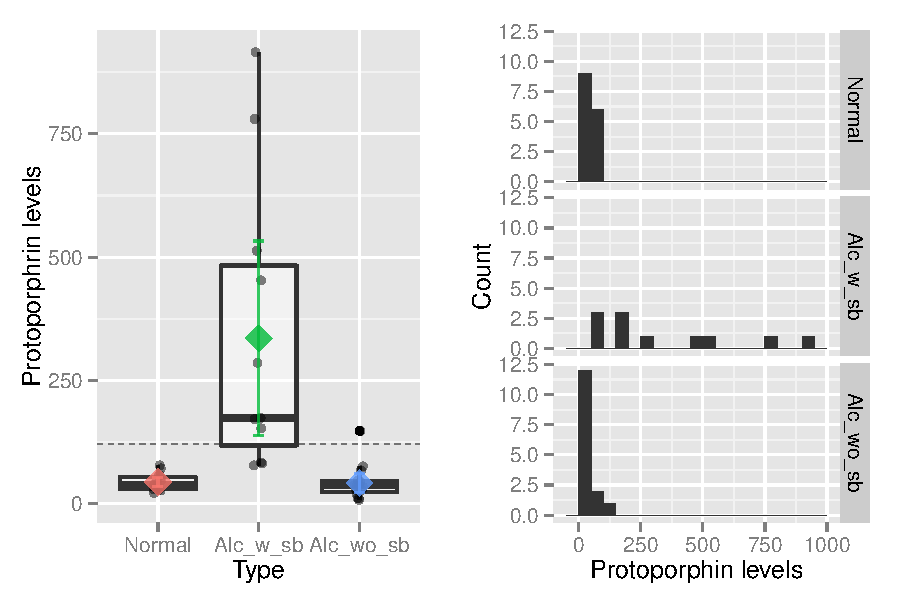
\includegraphics[width=\maxwidth]{figure/4_a_plot-1} 

}



\end{knitrout}

\begin{knitrout}
\definecolor{shadecolor}{rgb}{0.969, 0.969, 0.969}\color{fgcolor}\begin{kframe}
\begin{alltt}
\hlcom{#statistical summary of each type}
\hlkwd{by}\hlstd{(proto.long}\hlopt{$}\hlstd{level, proto.long}\hlopt{$}\hlstd{type, summary)}
\end{alltt}
\begin{verbatim}
## proto.long$type: Normal
##    Min. 1st Qu.  Median    Mean 3rd Qu.    Max. 
##   22.00   30.00   39.00   44.27   54.50   78.00 
## -------------------------------------------------------- 
## proto.long$type: Alc_w_sb
##    Min. 1st Qu.  Median    Mean 3rd Qu.    Max. 
##    78.0   118.5   174.0   335.5   483.0   915.0 
## -------------------------------------------------------- 
## proto.long$type: Alc_wo_sb
##    Min. 1st Qu.  Median    Mean 3rd Qu.    Max. 
##    8.00   24.00   37.00   42.53   46.00  148.00
\end{verbatim}
\begin{alltt}
\hlkwd{by}\hlstd{(proto.long}\hlopt{$}\hlstd{level, proto.long}\hlopt{$}\hlstd{type,} \hlkwa{function}\hlstd{(}\hlkwc{X}\hlstd{) \{}\hlkwd{c}\hlstd{(}\hlkwd{IQR}\hlstd{(X),} \hlkwd{sd}\hlstd{(X),} \hlkwd{length}\hlstd{(X))\})}
\end{alltt}
\begin{verbatim}
## proto.long$type: Normal
## [1] 24.50000 16.79909 15.00000
## -------------------------------------------------------- 
## proto.long$type: Alc_w_sb
## [1] 364.5000 293.4459  11.0000
## -------------------------------------------------------- 
## proto.long$type: Alc_wo_sb
## [1] 22.00000 34.94254 15.00000
\end{verbatim}
\end{kframe}
\end{knitrout}


\begin{knitrout}
\definecolor{shadecolor}{rgb}{0.969, 0.969, 0.969}\color{fgcolor}\begin{kframe}
\begin{alltt}
\hlcom{# kruskal-Wallis test with equal variance}
\hlstd{fit.proto} \hlkwb{<-} \hlkwd{kruskal.test}\hlstd{(level} \hlopt{~} \hlstd{type,} \hlkwc{data} \hlstd{= proto.long)}
\hlstd{fit.proto}
\end{alltt}
\begin{verbatim}
## 
## 	Kruskal-Wallis rank sum test
## 
## data:  level by type
## Kruskal-Wallis chi-squared = 23.1182, df = 2, p-value = 9.549e-06
\end{verbatim}
\begin{alltt}
\hlcom{#group comparisons}
\hlcom{#WILCOXON-MANN-WHITNEY test of equal population dedians}
\hlkwd{wilcox.test}\hlstd{(proto}\hlopt{$}\hlstd{Normal, proto}\hlopt{$}\hlstd{Alc_w_sb,} \hlkwc{conf.int} \hlstd{=} \hlnum{TRUE}\hlstd{)}
\end{alltt}
\begin{verbatim}
## 
## 	Wilcoxon rank sum test with continuity correction
## 
## data:  proto$Normal and proto$Alc_w_sb
## W = 0.5, p-value = 2.324e-05
## alternative hypothesis: true location shift is not equal to 0
## 95 percent confidence interval:
##  -435.00001  -61.99995
## sample estimates:
## difference in location 
##                   -144
\end{verbatim}
\begin{alltt}
\hlkwd{wilcox.test}\hlstd{(proto}\hlopt{$}\hlstd{Normal, proto}\hlopt{$}\hlstd{Alc_wo_sb,} \hlkwc{conf.int} \hlstd{=} \hlnum{TRUE}\hlstd{)}
\end{alltt}
\begin{verbatim}
## 
## 	Wilcoxon rank sum test with continuity correction
## 
## data:  proto$Normal and proto$Alc_wo_sb
## W = 137.5, p-value = 0.3093
## alternative hypothesis: true location shift is not equal to 0
## 95 percent confidence interval:
##  -8.000014 21.000040
## sample estimates:
## difference in location 
##               8.000074
\end{verbatim}
\begin{alltt}
\hlkwd{wilcox.test}\hlstd{(proto}\hlopt{$}\hlstd{Alc_wo_sb, proto}\hlopt{$}\hlstd{Alc_w_sb,} \hlkwc{conf.int} \hlstd{=} \hlnum{TRUE}\hlstd{)}
\end{alltt}
\begin{verbatim}
## 
## 	Wilcoxon rank sum test with continuity correction
## 
## data:  proto$Alc_wo_sb and proto$Alc_w_sb
## W = 3, p-value = 4.117e-05
## alternative hypothesis: true location shift is not equal to 0
## 95 percent confidence interval:
##  -442.00000  -71.99999
## sample estimates:
## difference in location 
##                   -146
\end{verbatim}
\end{kframe}
\end{knitrout}

\subsection{Analysis of Log Transformed Data}

\begin{knitrout}
\definecolor{shadecolor}{rgb}{0.969, 0.969, 0.969}\color{fgcolor}\begin{kframe}
\begin{alltt}
\hlcom{#create log transformed data}
\hlstd{proto.long}\hlopt{$}\hlstd{log} \hlkwb{<-} \hlkwd{log}\hlstd{(proto.long}\hlopt{$}\hlstd{level)}
\hlcom{#create box plot}
\hlstd{proto.log.p} \hlkwb{<-} \hlkwd{ggplot}\hlstd{(proto.long,} \hlkwd{aes}\hlstd{(}\hlkwc{x} \hlstd{= type,} \hlkwc{y} \hlstd{= log))}
\hlstd{proto.log.p} \hlkwb{<-} \hlstd{proto.log.p} \hlopt{+} \hlkwd{geom_hline}\hlstd{(}\hlkwc{yintercept} \hlstd{=} \hlkwd{mean}\hlstd{(proto.long}\hlopt{$}\hlstd{log),} \hlkwc{color} \hlstd{=} \hlstr{"black"}\hlstd{,}
                              \hlkwc{linetype} \hlstd{=} \hlstr{"dashed"}\hlstd{,} \hlkwc{size} \hlstd{=} \hlnum{0.3}\hlstd{,}  \hlkwc{alpha} \hlstd{=} \hlnum{0.5}\hlstd{)}
\hlstd{proto.log.p} \hlkwb{<-} \hlstd{proto.log.p} \hlopt{+} \hlkwd{geom_boxplot}\hlstd{(}\hlkwc{size} \hlstd{=} \hlnum{0.75}\hlstd{,} \hlkwc{alpha} \hlstd{=} \hlnum{0.5}\hlstd{)} \hlcom{# boxplot}
\hlstd{proto.log.p} \hlkwb{<-} \hlstd{proto.log.p} \hlopt{+} \hlkwd{geom_point}\hlstd{(}\hlkwc{position} \hlstd{=} \hlkwd{position_jitter}\hlstd{(}\hlkwc{w} \hlstd{=} \hlnum{0.05}\hlstd{,} \hlkwc{h} \hlstd{=} \hlnum{0}\hlstd{),}
                              \hlkwc{alpha} \hlstd{=} \hlnum{0.5}\hlstd{,} \hlkwc{size} \hlstd{=} \hlnum{2}\hlstd{)}
\hlstd{proto.log.p} \hlkwb{<-} \hlstd{proto.log.p} \hlopt{+} \hlkwd{stat_summary}\hlstd{(}\hlkwc{fun.y} \hlstd{= mean,} \hlkwc{geom} \hlstd{=} \hlstr{"point"}\hlstd{,} \hlkwc{shape} \hlstd{=} \hlnum{18}\hlstd{,}
                                \hlkwc{size} \hlstd{=} \hlnum{6}\hlstd{,} \hlkwd{aes}\hlstd{(}\hlkwc{color} \hlstd{= type),} \hlkwc{alpha} \hlstd{=} \hlnum{0.8}\hlstd{)}
\hlstd{proto.log.p} \hlkwb{<-} \hlstd{proto.log.p} \hlopt{+} \hlkwd{stat_summary}\hlstd{(}\hlkwc{fun.data} \hlstd{=} \hlstr{"mean_cl_normal"}\hlstd{,} \hlkwc{geom} \hlstd{=} \hlstr{"errorbar"}\hlstd{,}
                                \hlkwc{width} \hlstd{=} \hlnum{.1}\hlstd{,} \hlkwd{aes}\hlstd{(}\hlkwc{color} \hlstd{= type),} \hlkwc{alpha} \hlstd{=} \hlnum{0.8}\hlstd{)}
\hlstd{proto.log.p} \hlkwb{<-} \hlstd{proto.log.p} \hlopt{+} \hlkwd{labs}\hlstd{(}\hlkwc{y} \hlstd{=}\hlstr{"Protoporphrin levels"}\hlstd{,}\hlkwc{x} \hlstd{=} \hlstr{"Type"}\hlstd{)}
\hlstd{proto.log.p} \hlkwb{<-} \hlstd{proto.log.p} \hlopt{+} \hlkwd{guides}\hlstd{(}\hlkwc{color} \hlstd{=} \hlnum{FALSE}\hlstd{)}

\hlcom{# create histograms}
\hlstd{proto.log.hist} \hlkwb{<-} \hlkwd{ggplot}\hlstd{(proto.long,} \hlkwd{aes}\hlstd{(}\hlkwc{x} \hlstd{= log))} \hlopt{+} \hlkwd{geom_histogram}\hlstd{(}\hlkwc{binwidth} \hlstd{=} \hlnum{.5}\hlstd{)}
\hlstd{proto.log.hist} \hlkwb{<-} \hlstd{proto.log.hist} \hlopt{+} \hlkwd{facet_grid}\hlstd{(type} \hlopt{~} \hlstd{.)}
\hlstd{proto.log.hist} \hlkwb{<-} \hlstd{proto.log.hist} \hlopt{+} \hlkwd{labs}\hlstd{(}\hlkwc{y} \hlstd{=} \hlstr{"Count"}\hlstd{,} \hlkwc{x} \hlstd{=} \hlstr{"Protoporphin levels"}\hlstd{)}
\hlcom{# plot boxplot and historgram}
\hlkwd{grid.arrange}\hlstd{(proto.log.p, proto.log.hist,} \hlkwc{ncol} \hlstd{=} \hlnum{2}\hlstd{)}
\end{alltt}
\end{kframe}

{\centering 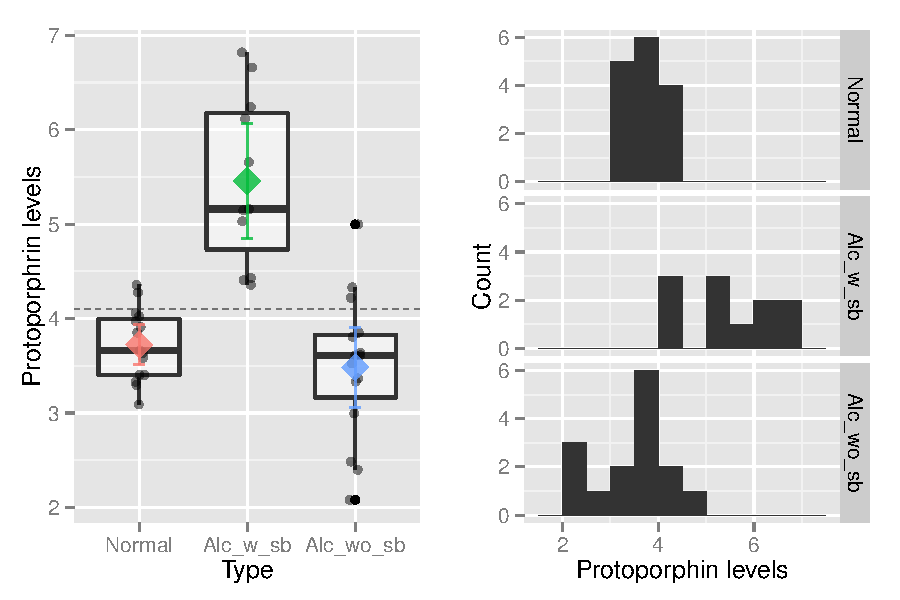
\includegraphics[width=\maxwidth]{figure/4_a_plot_log-1} 

}



\end{knitrout}

\begin{knitrout}
\definecolor{shadecolor}{rgb}{0.969, 0.969, 0.969}\color{fgcolor}\begin{kframe}
\begin{alltt}
\hlcom{#statistical summary of log transformed data}
\hlkwd{by}\hlstd{(proto.long}\hlopt{$}\hlstd{log, proto.long}\hlopt{$}\hlstd{type, summary)}
\end{alltt}
\begin{verbatim}
## proto.long$type: Normal
##    Min. 1st Qu.  Median    Mean 3rd Qu.    Max. 
##   3.091   3.401   3.664   3.724   3.998   4.357 
## -------------------------------------------------------- 
## proto.long$type: Alc_w_sb
##    Min. 1st Qu.  Median    Mean 3rd Qu.    Max. 
##   4.357   4.731   5.159   5.457   6.178   6.819 
## -------------------------------------------------------- 
## proto.long$type: Alc_wo_sb
##    Min. 1st Qu.  Median    Mean 3rd Qu.    Max. 
##   2.079   3.164   3.611   3.483   3.828   4.997
\end{verbatim}
\begin{alltt}
\hlkwd{by}\hlstd{(proto.long}\hlopt{$}\hlstd{log, proto.long}\hlopt{$}\hlstd{type,} \hlkwa{function}\hlstd{(}\hlkwc{X}\hlstd{) \{}\hlkwd{c}\hlstd{(}\hlkwd{IQR}\hlstd{(X),} \hlkwd{sd}\hlstd{(X),} \hlkwd{length}\hlstd{(X))\})}
\end{alltt}
\begin{verbatim}
## proto.long$type: Normal
## [1]  0.5966244  0.3778145 15.0000000
## -------------------------------------------------------- 
## proto.long$type: Alc_w_sb
## [1]  1.4474566  0.9011606 11.0000000
## -------------------------------------------------------- 
## proto.long$type: Alc_wo_sb
## [1]  0.6644367  0.7685407 15.0000000
\end{verbatim}
\end{kframe}
\end{knitrout}


\begin{knitrout}
\definecolor{shadecolor}{rgb}{0.969, 0.969, 0.969}\color{fgcolor}\begin{kframe}
\begin{alltt}
\hlcom{# ANOVA on log transformed data}
\hlstd{fit.proto.log} \hlkwb{<-} \hlkwd{aov}\hlstd{(log} \hlopt{~} \hlstd{type,} \hlkwc{data} \hlstd{= proto.long)}
\hlkwd{summary}\hlstd{(fit.proto.log)}
\end{alltt}
\begin{verbatim}
##             Df Sum Sq Mean Sq F value   Pr(>F)    
## type         2  28.07  14.035      29 2.25e-08 ***
## Residuals   38  18.39   0.484                     
## ---
## Signif. codes:  0 '***' 0.001 '**' 0.01 '*' 0.05 '.' 0.1 ' ' 1
\end{verbatim}
\begin{alltt}
\hlcom{# from long to wide}
\hlstd{proto.wide} \hlkwb{<-} \hlkwd{dcast}\hlstd{(proto.long, row} \hlopt{~} \hlstd{type,} \hlkwc{value.var} \hlstd{=} \hlstr{"log"}\hlstd{)}

\hlcom{# Tukey}
\hlkwd{TukeyHSD}\hlstd{(fit.proto.log)}
\end{alltt}
\begin{verbatim}
##   Tukey multiple comparisons of means
##     95% family-wise confidence level
## 
## Fit: aov(formula = log ~ type, data = proto.long)
## 
## $type
##                          diff        lwr        upr     p adj
## Alc_w_sb-Normal     1.7326582  1.0592061  2.4061103 0.0000007
## Alc_wo_sb-Normal   -0.2406837 -0.8601695  0.3788021 0.6140177
## Alc_wo_sb-Alc_w_sb -1.9733419 -2.6467940 -1.2998898 0.0000000
\end{verbatim}
\end{kframe}
\end{knitrout}


\begin{itemize}
\item \textbf{Graphical Summary:}  Considering either the mean or the median, the typical
protoporphin level increases dramatically when sideroblasts are present, where protoporphin
levels in the normal and alcoholic populations appear similar.  Additionally, the IQR and
standard deviation in protoporhin levels is substantially greater in the population with
sideroblasts than those populations without sideroblasts.  The difference in the means,
medians, and variance appears substantial across the three populations.\

The log transformed data have much less spread and variances that are far more consistent
across the three populations.  The log transformation did not alter the order of
respecstive values for mean and median.


\item \textbf{Kruskal-Wallis ANOVA:} Let $\eta_0$ be the median protoporphin level in a
normal population and define $\eta_1$ and $\eta_2$ as the median protoporpin level in a
population of alcoholics with sideroblasts and a population of alcoholics in without
sideroblasts.  We are interested in if it is plausible that the
difference in the median protophorphin levels across three populations is equal.  In notation,
$H_0: \eta_1 = \eta_2 = \eta_3 $ against $H_A:$ not $H_0$.
The p-value from this test was $9.5*10^{-6}$, which is less than 0.05; therefore, I reject
the null hypothesis in favor of the alternative.


\item \textbf{Assumptions of Kruskal-Wallis:} These methods assumed that independent random samples from
two populations were utilized and that the samples came from populations having
an identical distribution, e.g., distributions with similar shape and spread.

\item \textbf{Groupings from Wicoxon Rank Tests:}
\begin{verbatim}
Alc_wo_sb   Normal   Alc_w_sb
------------------   -------
\end{verbatim}

\item \textbf{ANOVA of Log Transformed Data:} Let $\mu_0$ be the mean protoporphin level in a
normal population and define $\mu_1$ and $\mu_2$ as the mean protoporpin level in a
population of alcoholics with sideroblasts and a population of alcoholics in without
sideroblasts.  We are interested in if it is plausible that the
difference in the mean protophorphin levels across three populations is equal.  In notation,
$H_0: \mu_1 = \mu_2 = \mu_3 $ against $H_A:$ not $H_0$.The p-value from this test was
$2.3*10^{-5}$, which is less than 0.05; therefore, I reject
the null hypothesis in favor of the alternative.

\item \textbf{Assumptions of ANOVA:} These methods assumed that independent random samples from
two populations were utilized and
that the samples came from populations with normal distributions having similar variance.

\item \textbf{Groupings from Tukey HSD}
\begin{verbatim}
Alc_wo_sb   Normal   Alc_w_sb
------------------   -------
\end{verbatim}


\item \textbf{Conclusions:} Based on the non parametric Kruskal-Wallis ANOVA of the untransformed data
and the parametric ANOVA of the log transformed data, both the median and mean protoporphin levels
are different across the three populations.  The different analysis methods resulted in
similar groupings where the normal and alcoholic with out sideroblasts  populations had
similar means and medians at the 5\% levels, and the alcoholic with sideroblasts population
had a different mean and median from the other two populations at the 5\% level.

\end{itemize}
\end{document}
